\section{Experiments}
\label{sec:exp}

The purpose of this experiment is to implement a few example generalized critics and compare the performance against that of a single critic. Specifically, we want to check how each of the tested environments reacts to the implemented method, what are the effects of changing the $\lambda$ coefficient in different estimations of the advantage, and how the average return is affected by the aggregation function.

\subsection{Experiment Setting}
% In the case of a continuous action space, $\pi$ is a gaussian distribution. <- add this to experiments
For the sake of this experiment, we will use continuous control tasks from the OpenAI Gym \cite{brockman2016openai} toolkit collection. In particular, we use the variants that are based on the Bullet physics engine from the Pybullet \cite{coumans2019pybullet} package: AntBulletEnv-v0, Walker2DBulletEnv-v0 and HumanoidBulletEnv-v0. Those environments are simulated with the Bullet free physics engine.

The experiment setting is as follows: for every run, we implement a generalized critic with two values for the advantage function based on the same estimate of $V(s_t)$ by calculating a GAE function with different values for the $\lambda$ coefficient. The aggregation function in this case is defined as a convex combination, with a weight vector $\beta$. The final critic value is given as follows

\[ \mathcal{F}(\hat{A}_1^{GAE(\gamma, \lambda_1)}, \hat{A}_2^{GAE(\gamma, \lambda_2)}) = \beta_1\hat{A}_1^{GAE(\gamma, \lambda_1)}+\beta_2\hat{A}_2^{GAE(\gamma, \lambda_2)} \]

such that $\beta_1 + \beta_2 = 1$.

We conduct two sets of experiments: 
\begin{enumerate}
\item To observe the effect of the critic on each of the environments, we set $\beta=(0.5, 0.5)$ and experiment with two generalized critics with their vectors of $\lambda$ values corresponding to (0.97, 0.93) and (0.99, 0.97) respectively. (results reported in table \ref{tab:reslam}
\item For one of the previous generalized critics ($\lambda = (0.97, 0.93)$), we test three different aggregation function such that $\beta_1 = (0.5, 0.5)$, $\beta_2 = (0.75, 0.25)$ and $\beta_3 = (0.25, 0.75)$ (results in figure \ref{fig:res})
\end{enumerate}
The basic critic compared against in each case uses the default value $\lambda = 0.97$.

The policy optimization method that we use for this experiment is the clipping variant of Proximal Policy Optimization~\cite{schulman2017proximal}. The policy update is performed as follows:
\begin{align*}
\theta_{k+1} = & \arg \max_{\theta} \frac{1}{| \mathcal{D}_k | T} \sum_{\tau \in \mathcal{D}_k} \sum_{t=0}^T \\ 
& \min \left(\frac{\pi_{\theta}(a_t\bar s_t)}{\pi_{\theta_k}(a_t\bar s_t)} A^{\pi_{\theta_k}}(a_t, s_t), g(\epsilon, A^{\pi_{\theta_k}}(a_t, s_t))\right)
\end{align*}

We use OpenAI's ``Spinning Up'' baseline implementation \cite{achiam2018openai} as a benchmark, as the codebase is well maintained and seems to perform at least as well as other reference codebases. Our work only focuses on the tensorflow implementation so the reported numbers may not apply to the newly added pytorch version.
\subsection{Experiment Results}

Table \ref{tab:reslam} shows the average returns over 5 random seeds for each generalized critic variant after two million timesteps. The results are rounded to the second decimal.

We notice that the Humanoid environment (Figure~\ref{fig:res}~(b)) is mostly indifferent to either a change in the number of critics or in the aggregation function, and performs on average in the same way. Both the Walker2D and the Ant environments (Figure~\ref{fig:res}, (a) and (c) respectively) show a certain sensitivity to either changes and a tendency to improve considerably for a few given values. It is interesting to note that the optimal hyperparameters for each case are not the same. This highlights the need for an aggregation function that is trained from sampled environment data rather than a pre-defined function.

\begin{table}[!htb]
\begin{tabular}{p{22mm}p{14mm}p{15mm}p{11mm}}
Algorithm & Walker2D & Ant & Humanoid \\
PPO ($\lambda$ = 0.97) & 690.47 & 1107.71 & \textbf{110.85} \\
\hline
$\lambda$ = (0.97, 0.93) & 718.80 & \textbf{1535.21} & 108.23  \\ 
\hline
$\lambda$ = (0.99, 0.97)& \textbf{752} & 1080.83 & 106.99 \\ 
\end{tabular}
\caption{Performance for three generalized critics across environments}
\label{tab:reslam}
\end{table}

% Below is an example of how to insert images. Delete the ``\vspace'' line,
% uncomment the preceding line ``\centerline...'' and replace ``imageX.ps''
% with a suitable PostScript file name.
% -------------------------------------------------------------------------
\begin{figure}[!htb]

\begin{minipage}[b]{.48\linewidth}
  \centering
  \centerline{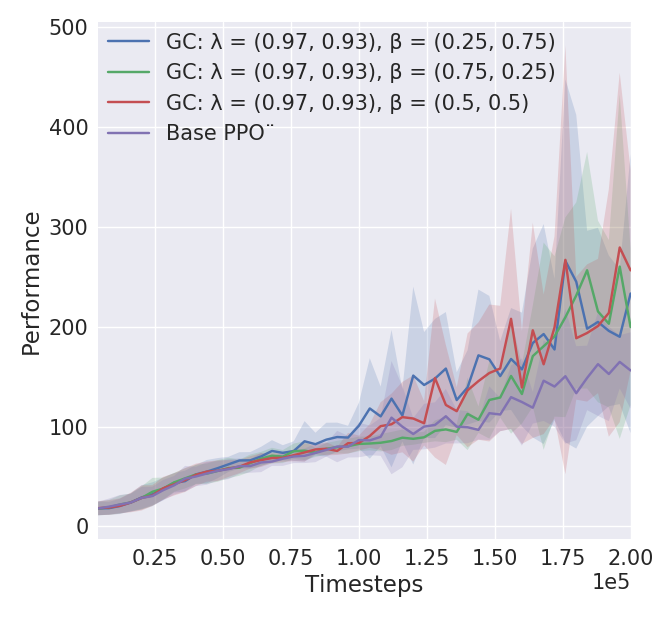
\includegraphics[width=4.0cm]{images/WalkerCoef}}
%  \vspace{2.0cm}
  \centerline{(a) Walker2DBulletEnv-v0}\medskip
\end{minipage}
\begin{minipage}[b]{.48\linewidth}
  \centering
  \centerline{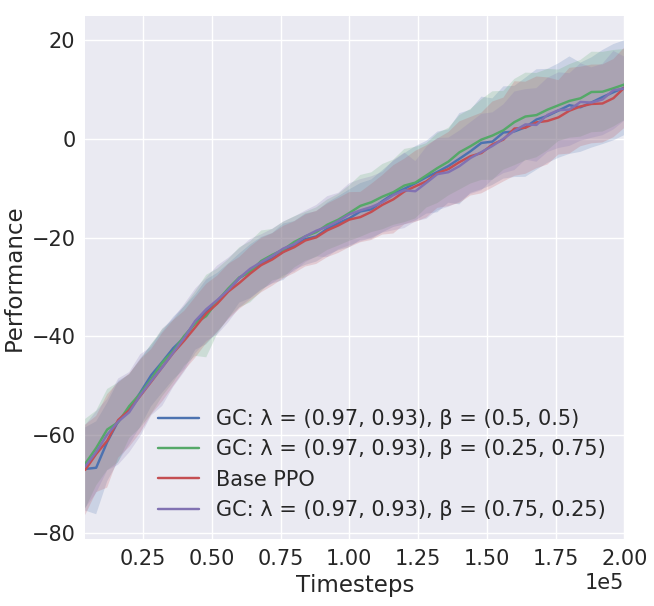
\includegraphics[width=4.0cm]{images/HumanoidCoef}}
%  \vspace{2.0cm}
  \centerline{(b) HumanoidBulletEnv-v0}\medskip
\end{minipage}

%
\begin{minipage}[b]{\linewidth}
  \centering
  \centerline{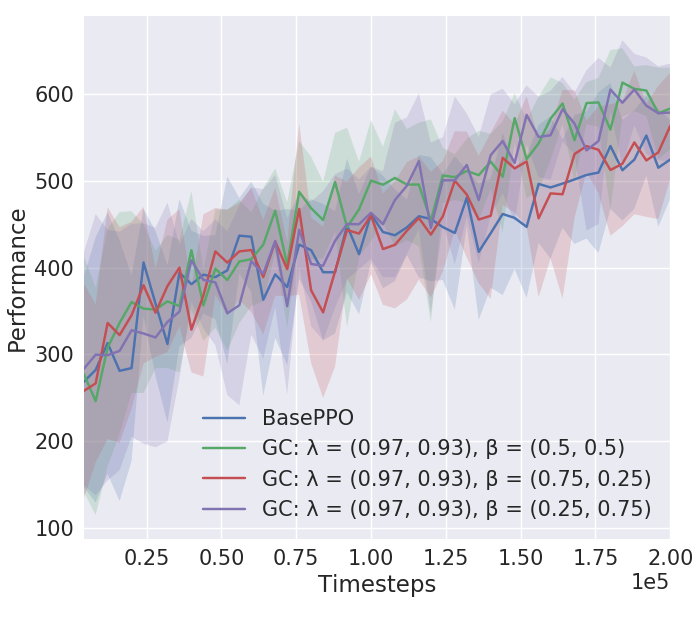
\includegraphics[width=4.0cm]{images/AntCoef}}
%  \vspace{1.5cm}
  \centerline{(c) AntBulletEnv-v0}\medskip
\end{minipage}
%\hfill
%\begin{minipage}[b]{0.48\linewidth}
%  \centering
%  \centerline{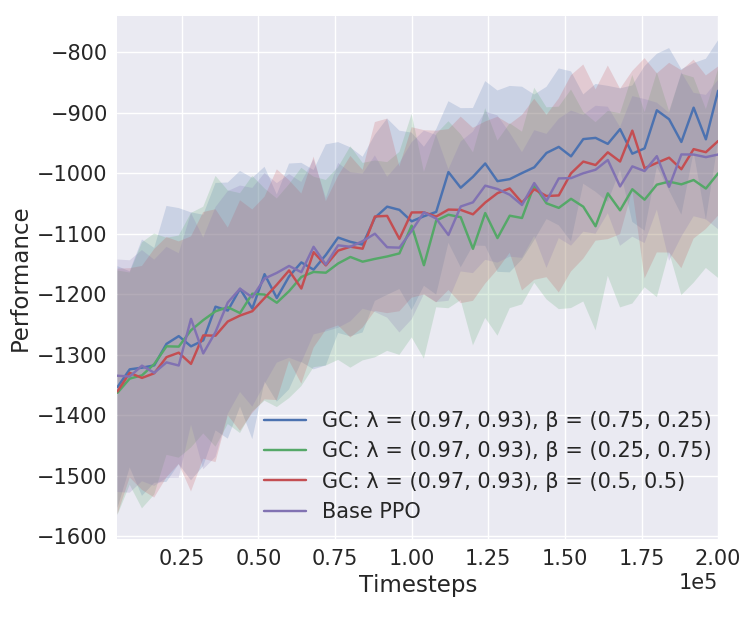
\includegraphics[width=4.0cm]{images/PendulumCoef}}
%  \vspace{1.5cm}
%  \centerline{(d) Pendulum}\medskip
%\end{minipage}
%
\caption{Performance of different coefficients for the aggregation function across environments.}
\label{fig:res}
%
\end{figure}


% To start a new column (but not a new page) and help balance the last-page
% column length use \vfill\pagebreak.
% -------------------------------------------------------------------------
%\vfill
%\pagebreak

